
\chapter{The transmission of the Welsh laws}
\label{cha:welsh-laws}

\section{Some quotes, tables, and stemmas}
\label{sec:some-quotes-tables}


% \tqt{One advantage which Welsh law enjoyed in the political storms of the thirteenth century was that it had a written form. Already in the twelfth century it was felt to be an embarassment if law remained unwritten. Roman law was embodied in texts, and with the great legal revival of the eleventh and twelfth centuries it was felt that any law worthy of the name should be written.
% }{charles-edwards_welsh_1989}{14}

\tqt{Welsh law survives in many complete manuscripts and fragments of others. The difficulty scholars have had in coping with this wealth of material stems from two opposite truths: first, each manuscript is an individual entity in that no one manuscript presents a text exactly the same as any other; but, secondly, the manuscripts fall into groups because they share, to a greater or lesser extent, the same content. As a result there have been long terminological travails attempting to give due weight both to the variations between manuscripts and also the links between them.
}{charles-edwards_welsh_1989}{17}


\tqt{The considerable differences between the law books show that their authors were not concerned, like the Irish, to preserve intact a standard text handed down from the past.
  Linguistically, the laws are not unlike many Middle Welsh prose tales: in spite of the occasional early feature the language as a whole generally accords with the dates of the manuscripts.
}{charles-edwards_welsh_1989}{21--22}

% \tqt{{[T]}he distinction between the Versions and the Anomalous Laws lies in the existence of a certain pattern according to which it was thought that a wide-ranging account of the Law of Hywel ought to be constructed. The pattern was not immutable, as is shown by the creation of the Test Book in \textsc{Ior} or by the wide variations in the ordering of the tractates in \textsc{Cyfn}.}{charles-edwards_welsh_1989}{26}

\Textcite{wiliam_llyfr_1960} notes that, within \textit{B}, `[m]utations of initial consonants are sometimes indicated, sometimes not. The nasal mutation, however, is regularly shown.'~\autocite[xlii]{wiliam_llyfr_1960}.

\begin{figure}[h]
  \centering
  \begin{tikzpicture}[font=\itshape,level distance=10mm]
    \node(A){A}
    child {node {E}
      child [missing]
      child [missing]
      child {node(B) {B}}
    }
    child [missing]
    child {node(C) {C}}
    ;
    \draw(B)--(C)
    ;
    \node[right= 1em of C](S){\upshape saec.~XIII\textsuperscript{med}};
    \node[right= 5em of A]{c.~\upshape 1200};
    \node[right= 5em of B]{c.~\upshape 1282};
  \end{tikzpicture}
  \caption{Gwenogvryn Evans's \mw{Llyfr Iorwerth}, from \textcite{charles-edwards_textual_2016}.}
  \label{fig:gwevanslli}
\end{figure}

\begin{figure}[h]
  \centering
  \begin{tikzpicture}[font=\itshape]
    \node{X}
    child {node(alph) {α}
      child {node(B) {B}}
    }
    child {node (beta) {β}
      child {node(C) {C}}
      child {node (gamma) {γ}
        child {node (delta) {δ}
          child{node{A}}
          child{node{E}}
        }
        child[missing]
        child {node (eps){ε}
          child {node{D}}
          child{node{ζ}
            child {node {Col}}
            child {node {\upshape Llanforda}}
          }
        }
      }
    }
    ;
    \node[left=of alph](nalph){Galanas B \upshape added};
    \node[left= of B](nB){{\upshape no} damweiniau};
    \node[below left= of C](nC){{\upshape no} damweiniau};
    \node[below left=of delta,align=left](ndelta){- {\upshape Pref.\ to Test Bk.}\\+ Br.\ Gwŷr Arfon};
    \node[right=of beta](nbeta){+ Galanas E \upshape\& Pref.\ to Test Book};
    \node[right=of gamma](ngamma){+ Damweiniau I};
    \node[right=of eps](neps){+ Damweiniau II};
    \draw[dotted](alph)--(nalph);
    \draw[dotted](B)--(nB);
    \draw[dotted](C)--(nC);
    \draw[dotted](delta)--(ndelta);
    \draw[dotted](beta)--(nbeta);
    \draw[dotted](gamma)--(ngamma);
    \draw[dotted](eps)--(neps);
  \end{tikzpicture}
  \caption{Wiliam's \mw{Llyfr Iorwerth}, simplified by \textcite{charles-edwards_textual_2016}.}
  \label{fig:wiliamiorwerth}
\end{figure}

%  \begin{figure}[h]
%     \centering
% \begin{tikzpicture}[font=\itshape]
% \node{\upshape Redaction I} 
% child {node {α}
%   child [level distance=15mm]{node {A}}
%   child [level distance=15mm]{node {E}}
% }
% child [xshift=1em]{node {\upshape Redaction II}
%   child [grow=down] {node {β}
%     child [level distance =10mm,xshift=-1em]{node {C}}
%     }
%     child[level distance=20mm] {node{γ}
%       child [level distance=15mm]{node {\vphantom{J}GDLew}}
%       child [level distance=15mm]{node{BJKTim}}
%     }
% }
%     ;
%   \end{tikzpicture}
%     \caption{A stemma of the Laws of the Country  according to Thomas Charles-Edwards.}
%     \label{fig:stemmalawc}
%   \end{figure}
  
  \begin{figure}[h]
    \centering
    \begin{tikzpicture}[font=\itshape,level distance=17.5mm]
\node(1){\upshape Redaction I} 
child {node {α}
  child{node(A) {A}}
  child{node(E) {E}}
}
child[missing]
child {node(2) {\upshape Redaction II}
  child {node[align=center] (beta){β}
    child [dashed,level distance=35mm]{node(B) {\vphantom{J}B}
      edge from parent node [midway,above,sloped]{Test Book}}
    child {node {C}}
    child[missing]
  }
  child[missing]
  child {node(gamma){γ}
    child  {node {GDLew}}
    child[missing]
      child [level distance=35mm]{node {JKTim}
      edge from parent node (J){}  
      }
  }
}
  ;
  \node[above left=of E](nA){Bees I \& II};
  \node[below left=of beta,xshift=-15mm](nbeta){Bees I};
  \node[right=of 1](n1){Bees I \& II};
  \node[right=of 2,align=center](n2){+ Preface to Test Book\\ Bees I \& II};
  \node[right=of gamma,align=center](ngamma){+ Hywel to Rome\\Bees II};
  \draw[dotted](A)--(nA) -- (E);
  \draw[dotted](beta)--(nbeta);
  \draw[dotted](1)--(n1);
  \draw[dotted](2)--(n2);
  \draw[dotted](gamma)--(ngamma);
  \draw[dashed](B) to  node [midway,below,sloped]{Laws of Country}  (J);
\end{tikzpicture}
\caption{A stemma of \mw{Llyfr Iorwerth} manuscripts according to \textcite{charles-edwards_textual_2016}. Dashed lines indicate partial transmission.}
\label{fig:stemmatestb}
\end{figure}

\begin{figure}[h]
  \centering
  \begin{tikzpicture}[font=\itshape]
    \node{X}
    child{node{α}
      child{node{γ}
        child{node{A}}
        child{node{E}}
      }
      child{node{C}}
    }
    child[missing]
    child{node{β}
      child{node{δ}
        child{node{D}}
        child{node{Lew}}
      }
      child[missing]
      child{node{ε}
        child{node{G}}
        child{node{ζ}
          child{node{J}}
          child{node{B}}
          child{node{K}}
          child{node{Tim}}
        }
      }
    }
  ;
  \end{tikzpicture}
  \caption{Stemma of Ior's tractate on suretyship \autocite[138]{charles-edwards_lawyers_1986}}
  \label{fig:suretyshstemma}
\end{figure}



\begin{spacing}{1}
  \itshape
  \begin{pages}
    \begin{Leftside}
      \beginnumbering
      \pstart[
      \subsection*{C 180ra1--180va23}
      \label{sec:parallel-text-c-1}
      ]
      \textup{/180ra/} Hewel \al{ỽ}ap kadell \al{t}ewyssaỽc kemry a deỽynnỽs attaỽ chwe gwyr o \al{p}ob kantref eg kemry oll hyt e ty gwyn en dyỽet a henny or gwyr doethaf en e \al{k}eỽoeth. e pedwar onadỽnt en llegyon ar deỽ en escolheygyon. Sef achaỽs e dwcpwyt er escolheygyon rac dody or lleegyon petheỽ a \al{ỽ}ey en erbyn er escrethỽr \al{g}lan. Ac esef amser e doethant eno petheỽnos amys \al{g}arawys. ac esef achaỽs e doethant eno e \al{g}arawys ỽrth na dely nep na dewedwyt kam nay \al{g}wneỽthỽr en er amser gleyndyt hỽnnỽ.
      \pend
      \pstart
      Ac ena ed edrychassant e kyỽreythyeỽ. ar hon a \al{ỽ}ey re \al{t}rom onadỽnt y hescaỽynhaỽ. ar hon a \al{ỽ}ey re eskaỽyn onadỽnt yhachwanegỽ. Peth or kyỽreythyeỽ a \al{a}dassant \al{ỽ}al ed oeydynt. peth arall a \al{ỽ}ynnassant y emendaỽ. ereyll a dyleassant \textup{/180rb/} en \al{k}ỽbyl. ac ereyll o newyd a \al{o}ssodassant.
      \pend
      \pstart
      Ac ena e dodassant hewel a henny o doethyon eỽ hemendyth ar nep a \al{k}amarỽerey or kyỽreythyeỽ henny ac ar er arglwyd ay semỽtey yr ỽn onadỽnt namyn kan dỽỽndep kynnỽlleytỽa \al{k}ymeynt ac a \al{w}u eno. ER eyl emendyth a dodassant ar er arglwyd ay rodey. ac ar e dyn ay kymerey \al{t}eylygdaỽt egneydyaeth ar ny \al{g}wyney teyr koloỽyn kyỽreyth a gwerth gwyllt a dof. ac a \al{p}erthyn attadỽnt
      \pend
      \pstart
      \pend
      \pstart
      Pwy \al{b}ynnac a \al{ỽ}ynho kymryt egneydyaeth \al{ỽ}al hy e mae yaỽn ydaỽ gwybot e llyỽyr hỽn. \al{ỽ}al e bo teylỽng. ydaỽ kymryt egneydyaeth. a phan \al{g}welo y athro y \al{ỽ}ot yn \al{t}eylỽng. ellyget ar er egnat llys ef. ar egnat llys \al{p}yeỽ y \al{p}roỽy. Ac os gwyl en \al{t}eylỽng enteỽ \al{p}yeỽ y ellỽng ef ar er arglwyd. ar arglwyd \al{p}yeỽ estynnỽ ydaỽ enteỽ egneydyaeth. ac en \al{ỽ}arnedyc e \al{ỽ}raỽt a \al{ỽ}arnho enteỽ o henny allan. Ac enteỽ \al{p}yeỽ rody pedeyr ar ỽgeynt yr egnat llys en y \al{o}byr. O derỽyd ydaỽ enteỽ barnỽ kam \al{ỽ}raỽt o henny allan ny dely enteỽ y \al{t}aỽaỽt \textup{/180va/} onys pryn yr y \al{w}erth kyỽreyth. O derỽyd emwystlaỽ ac enteỽ. ae \al{ỽ}ot enteỽ ar er yaỽn. ef adely wynepwarth y \al{g}an e nep a emwystlo ac ef. a chamlỽrỽ yr arglwyd. Ny dely egnat kymryt gwystyl onys myn ehỽn gwedy del oe \al{ỽ}raỽtle. ac ny dely kymryt y \al{g}an \al{l}eyc onyt kan adaỽ braỽt a \al{ỽ}o gwell y \al{g}an egnat arall nor hon a \al{ỽ}arnỽs ef.
      \pend
      \pstart
      Ar lleỽyr hỽn a \al{g}ynỽllỽs yorwerth \al{ỽ}ap madaỽc o \al{l}yỽyr kyỽnerth \al{ỽ}ap morgeneỽ. ac o \al{l}yỽyr gweyr \al{ỽ}ap rỽuaỽn. ac o \al{l}yỽyr Goronwy \al{ỽ}ap morydyc. ac y \al{g}yt a hennyor llyỽreỽ goreỽ a kaỽas heỽyt eg gwyned. a phowys. a deheỽparth. ar llyỽyr hỽn a \al{e}lwyr e llyỽyr praỽ. Sef ew henny teyr koloỽyn \al{k}yỽreyth. a gwerth gwyllt a dof. ac a \al{p}erthyn ar henny.
      \pend
      \endnumbering
    \end{Leftside}
    \begin{Rightside}
      \beginnumbering
      \pstart[
      \subsection*{D 55v20--57r2}
      \label{sec:d}
      ]
      \textup{/55v/} Howel \al{v}ab kadeỻ \al{t}ywyssaỽc kymry a dyuynnaỽd attaỽ chwe gwyr o \al{b}op kantref yng kymry hyt y ty gwynn yn dyuet. a hynny or gỽyr doethaf yn y \al{g}yuoeth. y pedwar onadunt yn ỻeygyon. ar deu yn yscolheigyon. \textup{/56r/} rac dodi or ỻeygyon petheu a \al{v}ei yn erbyn yr ysgruthyr \al{l}an. Sef amser y doethant yno; pythewnos a mis \al{g}arawys. ỽrth na dylyei neb na dywedut cam nae \al{w}neuthur yn yr amser gleindyt hỽnnỽ.
      \pend
      \pstart
      Ac yna yd edrychassant y kyfreitheu; yr honn a \al{v}ei ry \al{d}rom y chosp onadunt. y ỻeihau. ar honn a \al{v}ei ry \al{v}echan; y hachwanegu. Peth or kyfreitheu a \al{a}dassant \al{u}al yd yttoedynt peth araỻ a emendanassant. ereiỻ o \al{g}ỽbyl a dileassant.
      \pend
      \pstart
      ac yna y dodassant eu hemeỻtith howel a hynny o doethon ar yr arglỽyd a symuttei vn or kyfreitheu hynny; namyn \al{g}an duundeb kynnuỻeitua \al{g}ymeint a honno. ar eil emeỻtith a dodassant ar yr arglỽyd ae rodei. ac ar y dyn a \al{g}ymerei arnaỽ \al{d}eilygdaỽt ygneityaeth ar ny \al{w}ypei \al{t}eir kolofyn kyfreith. a gỽerth gỽyỻt a dof. ac a \al{b}erthyn attunt.
      \pend
      \pstart
      A gỽedy gỽneuthur ohonunt y kyfreitheu \al{u}al y tebygynt eu bot yn \al{d}eilỽg; yd aeth howel ac escob mynyỽ. ac escob assaf. ac escob bangor. ac y am hynny yny \al{v}u ar y \al{d}rydyd ar dec o athraỽon a doethon ereiỻ o \al{l}eygyon. ac yd aethant hyt yn ruuein. y \al{g}ymryt aỽdurdaỽt pab ruuein y \al{g}yfreitheu howel. ac yna y darỻewyt kyfreitheu howel rac bronn \al{p}ab ruuein. ac y bu \al{u}odlaỽn y pab udunt. ac y rodes y aỽdurdaỽt udunt. \textup{/56v/} ac y doeth howel ae \al{g}edymdeithon adref. Ac yr hynny hediỽ yd ydys yn daly o \al{g}yfreitheu hoỽel.
      \pend
      \pstart
      Pỽy \al{b}ynnac a \al{v}ynno kymryt ygneityaeth arnaỽ; \al{v}al hynn y mae idaỽ gỽybot y ỻyfyr hỽnn. \al{u}al y bo teilỽg idaỽ kymryt ygneityaeth. a phan \al{w}elo y athro y \al{v}ot yn \al{d}eilỽg; goỻyget ef att yr ygnat ỻys. ar ygnat ỻys \al{b}ieu y \al{b}roui. ac os gỽyl yn \al{d}eilỽg; ynteu \al{b}ieu y oỻỽg ef att yr arglỽyd. ar arglỽyd \al{b}ieu estynnu ygneityaeth idaỽ. ac yn \al{u}arnedic y \al{v}arn a \al{v}arnho o hynny aỻan. ac ynteu \al{b}ieu rodi pedeir ar hugeint yr ygnat ỻys yn y \al{o}byr. O deruyd idaỽ ynteu \al{v}arnu camvraỽt o hynny aỻan; ny dyly y \al{d}auaỽt ony s pryn yr y \al{w}erth kyfreith. O deruyd. ymwystlaỽ ac ynteu ae \al{v}ot ef ar yr iaỽn; ef a dyly wynebwerth y \al{g}an y neb a ymỽystlo ac ef. a chamlỽrỽ yr arglỽyd. Ny dyly ygnat kymryt gỽystyl gỽedy del oe \al{v}raỽtle. ony s mynn. ac ny dyly y \al{g}ymryt y \al{g}an \al{l}eyc; onyt \al{g}an adaỽ braỽt a \al{v}o gỽeỻ y \al{g}an araỻ nor \al{v}raỽt a \al{v}arnaỽd ef.
      \pend
      \pstart
      Y ỻyfyr hỽnn a \al{g}ynnuỻaỽd Jorwerth \al{u}ab madaỽc. o \al{l}yfyr kyfreith Morgeneu. a ỻyfyr gỽeir \al{u}ab ruaỽn. a ỻyfyr gronỽy \al{u}ab Moridic. ac y\al{g}yt a hynny or ỻyfreu goreu yg gỽyned. a phowys. a deheubarth. ar ỻyfyr hỽnn a \al{e}lwir ỻyfyr praỽf. Sef \textup{/57r/} yỽ hynny; teir kolofyn \al{k}yfreith. a gỽerth gỽyỻt a dof. ac a \al{b}erthyn ar hynny.
      \pend
      \endnumbering
    \end{Rightside}
  \end{pages} 
  \Pages
\end{spacing}

%%% Local Variables:
%%% mode: latex
%%% TeX-master: "../main"
%%% End:


\begin{figure}[h]
  \centering
  \begin{tabular}{cc}
I  & II\\
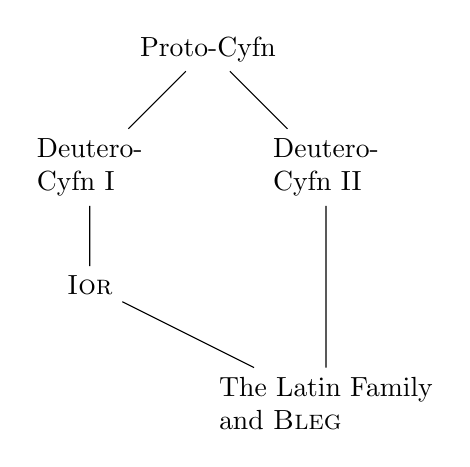
\begin{tikzpicture}[level distance=15mm,align=left]
\node(p){Proto-Cyfn}
child{node {Deutero-\\Cyfn I}
  child{node(ior){\textsc{Ior}}}
}
child[missing]
child {node {Deutero-\\Cyfn II}
  child[level distance=30mm] {node(lat){The Latin Family\\ and \textsc{Bleg}}}
}
;
\draw(ior)--(lat);    
\end{tikzpicture}
   &
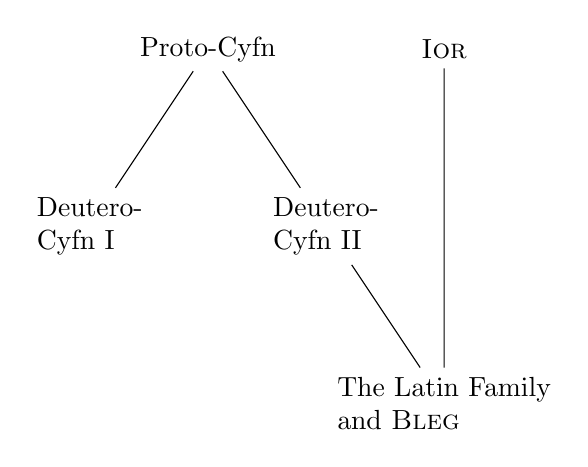
\begin{tikzpicture}[level distance=22.5mm,align=left]
\node(p){Proto-Cyfn}
child{node {Deutero-\\Cyfn I}
}
child[missing]
child {node {Deutero-\\Cyfn II}
  child[xshift=15mm] {node(lat){The Latin Family\\ and \textsc{Bleg}}}
}
;
\node[xshift=30mm](ior){\vphantom{J}\textsc{Ior}};
\draw(ior)--(lat);
\end{tikzpicture}
\end{tabular}

\caption{Two possible family trees of the Welsh law books according to \textcite[48]{charles-edwards_welsh_1989}.}
\label{fig:lawfamilies}
\end{figure}

% \begin{table}[h]
%   \centering
%   \begin{tabular}{@{}ll@{}}
%     \toprule
%     \tch{Old} & \tch{New} \\
%     \midrule
%     Ɛ & Ep \\
%     Ð & Dd \\
%     Ā & As\\
%     \rotatebox[origin=c]{180}{ω}& Mor\\
%      & An \\
%     \bottomrule
%   \end{tabular}
% \caption{Sigla for the anomalous laws}
% \label{tab:sigla}
% \end{table}

\begin{table}[h]
\centering
  \renewcommand{\labelenumi}{\Roman{enumi}}
  \renewcommand{\labelenumii}{\arabic{enumii}}
  \renewcommand{\labelenumiii}{(\roman{enumiii})}
\begin{tabular}{@{}p{0.45\textwidth}p{0.45\textwidth}@{}}
  \toprule
  \tch{\itshape Mk:}&\tch{\textsc{Ior}:}\\\midrule
\begin{enumerate}
\item Prologue
\item Laws of Court
\item Laws of Country
  \begin{enumerate}
  \item The Three Columns of Law, the Nine Tongued-ones, the value of limbs, \mw{galanas} and \mw{sarhaed}
  \item Land
  \item Value of Wild and Tame
  \item Other Laws of Country
    \begin{enumerate}
    \item Corn-damage
    \item Suretyship
    \item Women
    \end{enumerate}
  \end{enumerate}
\item Triads
\end{enumerate}
&

\begin{enumerate}
\item Prologue
\item The Book of the Court (43/17 from Manuscript \textit{B})
\item The Laws of Country
  \begin{enumerate}
  \item The Nine Tongued-ones
  \item Women
  \item Injury to Animals
  \item Surety and Contract
  \item Church Protection
  \item Land
  \item Children and Paternity
  \end{enumerate}
\item The Test Book (colophon: 120/7)
  \begin{enumerate}
  \item The Three Columns of Law (colophon: 120/7)
  \item Value of Wild and Tame (and the Value of Trees)
  \end{enumerate}
\item Appendages to the Test Book:
  \begin{enumerate}
  \item Value of Houses and Equipment
  \item Joint-ploughing
  \item Corn-damage
  \end{enumerate}
\end{enumerate}\\\bottomrule
\end{tabular}
\caption{The main divisions of \textit{Mk} and \textsc{Ior} according to \textcite[27--28]{charles-edwards_welsh_1989}}
\label{tab:divisions}
\end{table}

\section{Research plan for the laws}
\label{sec:research-plan-laws}

What do I want to do?
I want to analyze where \lT\ was represented in the various law texts.

Why do I want to do this?
I want to see under what circumstances scribes copying manuscripts maintained or changed the non-representation of \lT.

Which period is suitable for this purpose?
I expect that most instances of \lT\ were represented by the mid-fourteenth century, so manuscripts up until this period are most useful to chart the change in orthography.
Later manuscripts may still show traces of the early orthography, and may thus also be included.
I will focus on the transmission of \mw{Llyfr Iorwerth}, because most of the oldest law manuscripts contain this law text.

How are various manuscripts related to each other?
It is nowadays thought that none of the earliest extant manuscripts is a direct ancestor of another extant copy.
One author who did think this was J.\ Gwenogvryn Evans (Figure~\ref{fig:gwevanslli}).
Rather, extant manuscripts are held to have common exemplars that no longer exist.
Figure~\ref{fig:stemmatestb} gives a stemma for the Iorwerth manuscripts (and some more manuscripts), and I will use this stemma as a point of departure for my own research.

Which manuscripts may be used for analysis?
One useful manuscript is \textit{A}, the \gls{bbch}, dating from around 1250. This manuscript is one of the oldest law manuscripts, and its orthography is very unusual.
Another useful manuscript is \textit{B}, which is also fairly old, and dates from the end of the thirteenth century.
Other thirteenth-century manuscripts shown in Figure~\ref{fig:stemmatestb}: \textit{EC};
early fourteenth century: \textit{G};
other manuscripts in this stemma are all later than the fourteenth century.
Some more useful manuscripts are: \textit{VW}, by scribe X86; \textit{Tr}, by Gwilym Was Da.

What sections of the law texts are useful for analysis?
Figure~\ref{fig:stemmatestb} shows that \textit{B} was  transmitted in part from several sources. This makes both the Test Book and the Laws of Country interesting targets for analysis, as the orthography of lenition may confirm or deny this peculiar reconstruction by Charles-Edwards.
Figure~\ref{fig:stemmatestb} also shows that different parts of the Test Book may have been added in intermediate stages between Redaction I and the extant manuscripts.
Comparison of these chunks with text found in all the manuscripts may prove useful in establishing at what point in time these chunks were added, and therefore when some of the hypothetical nodes in the stemma were written.

\subsection{Fleshed-out research plan}
\label{sec:fleshed-out-research}
I will take the tractate on suretyship for analysis.
This tractate is found in many manuscripts from the Iorwerth tradition, and those manuscripts vary in date of composition from the mid-thirteenth century to 1404. 
\begin{table}[h]
  \centering
  % Table generated by Excel2LaTeX from sheet 'Sheet3'
  \begin{tabular}{@{}lddl@{}}
\toprule
  & Begin & End & Date \\
\midrule
\gls{sA} & 43.22 & 49.17 & s.xiii med \\
\gls{sB} & 20r.22 & 24v.10 & s.xiii\textsuperscript{2} \\
\gls{sC} & 155va.10 & 162rb.17 & s.xiii med \\
\gls{sD} & 52.19 & 63.23 & ca.\ 1404 \\
\gls{sE} & 34.5 & 40.19 &  s.xiii\textsuperscript{2} \\
\gls{sG} & 20r.1 & 28r.4 & s.xiv\textsuperscript{1} \\
\textcite{owen_ancient_1841} &  \multicolumn{2}{c}{Venedotian Code II.\textsc{vi}} &  \\
\textcite{wiliam_llyfr_1960} & \S 58 &\S 67 &  \\
\bottomrule
\end{tabular}%
  \caption{The tractate on suretyship in various recensions of \mw{Llyfr Iorwerth}.}
  \label{tab:surety}
\end{table}

\begin{figure}[h]
  \centering
  \begin{tikzpicture}[font=\itshape,level distance=10mm]
    \node{X}
    child{node{α}
      child{node{γ}
        child[level distance=20mm]{node{\gls{sA}}}
        child[level distance=20mm]{node{\gls{sE}}}
      }
      child[level distance=30mm]{node{\gls{sC}}}
      child[missing]
    }
    child{node{β}
      child{node{δ}
        child[level distance=20mm]{node{\gls{sD}}}
      }
      child{node{ε}
        child[level distance=20mm]{node{\gls{sG}}}
        child{node{ζ}
          child{node(sB){\gls{sB}}}
        }
      }
    }
  ;
  \end{tikzpicture}
  \caption{\mw{Llyfr Iorwerth}'s tractate on suretyship following \textcite[138]{charles-edwards_lawyers_1986}, containing only manuscripts used.}
  \label{fig:suretyshstemma2}
\end{figure}

 \begin{figure}[h]
    \centering
\begin{tikzpicture}[font=\itshape,level distance=10mm]
\node{\upshape Redaction I} 
child {node {α}
  child [level distance=20mm]{node {A}}
  child [level distance=20mm]{node {E}}
}
child[missing]
child {node {\upshape Redaction II}
  child {node {β}
    child {node {C}}
    }
    child {node{γ}
      child {node {GD}}
      child {node{B}}
    }
}
    ;
  \end{tikzpicture}
    \caption{A stemma of the Laws of the Country  according to \textcite{charles-edwards_textual_2016} containing only manuscripts used.}
    \label{fig:stemmalawc}
  \end{figure}
\section{Some preliminary observations}
\label{sec:some-prel-observ}

MS \textit{B}, folio 42v, \S 104 has the following as the preface of the Test Book:
\mwcc[preftestb]{B 42v.}{Llyma e dechreu e Llyuer Prauf. Sef yu henne, teyr colouen keureyth guerth gyullt a dof ac a perthyn arnadunt.}{Here starts the Test Book. That is, three columns of law of wild and tame value, and what relates to them.}
Figure~\ref{fig:stemmatestb} shows that the preface to the Test Book was added as late as Redaction II.
This one line shown in Example~\ref{preftestb} shows lenition word-internally, and there are two examples  where word-initial lenition may be expected:, \mw[columns of law]{colouen keureyth}, with lenition following a feminine noun, and \mw[that relates]{a perthyn}, with lenition following the verbal particle.
As lenition  is not written here, we may assume that Redaction II was composed before lenition of voiceless stops was written.
This is unsurprising, as one of its manuscripts, \textit{C}, is dated as early as 1250.
This somewhat trivial example serves to demonstrate how combined knowledge of when which parts were added in a stemma and of the orthography of lenition may date hypothetical nodes in a stemma. 


\begin{spacing}{1}
  \itshape
  \begin{pages}
    \begin{Leftside}
      \beginnumbering
      \pstart[
      \subsection*{C 180ra1--180va23}
      \label{sec:parallel-text-c-1}
      ]
      \textup{/180ra/} Hewel \al{ỽ}ap kadell \al{t}ewyssaỽc kemry a deỽynnỽs attaỽ chwe gwyr o \al{p}ob kantref eg kemry oll hyt e ty gwyn en dyỽet a henny or gwyr doethaf en e \al{k}eỽoeth. e pedwar onadỽnt en llegyon ar deỽ en escolheygyon. Sef achaỽs e dwcpwyt er escolheygyon rac dody or lleegyon petheỽ a \al{ỽ}ey en erbyn er escrethỽr \al{g}lan. Ac esef amser e doethant eno petheỽnos amys \al{g}arawys. ac esef achaỽs e doethant eno e \al{g}arawys ỽrth na dely nep na dewedwyt kam nay \al{g}wneỽthỽr en er amser gleyndyt hỽnnỽ.
      \pend
      \pstart
      Ac ena ed edrychassant e kyỽreythyeỽ. ar hon a \al{ỽ}ey re \al{t}rom onadỽnt y hescaỽynhaỽ. ar hon a \al{ỽ}ey re eskaỽyn onadỽnt yhachwanegỽ. Peth or kyỽreythyeỽ a \al{a}dassant \al{ỽ}al ed oeydynt. peth arall a \al{ỽ}ynnassant y emendaỽ. ereyll a dyleassant \textup{/180rb/} en \al{k}ỽbyl. ac ereyll o newyd a \al{o}ssodassant.
      \pend
      \pstart
      Ac ena e dodassant hewel a henny o doethyon eỽ hemendyth ar nep a \al{k}amarỽerey or kyỽreythyeỽ henny ac ar er arglwyd ay semỽtey yr ỽn onadỽnt namyn kan dỽỽndep kynnỽlleytỽa \al{k}ymeynt ac a \al{w}u eno. ER eyl emendyth a dodassant ar er arglwyd ay rodey. ac ar e dyn ay kymerey \al{t}eylygdaỽt egneydyaeth ar ny \al{g}wyney teyr koloỽyn kyỽreyth a gwerth gwyllt a dof. ac a \al{p}erthyn attadỽnt
      \pend
      \pstart
      \pend
      \pstart
      Pwy \al{b}ynnac a \al{ỽ}ynho kymryt egneydyaeth \al{ỽ}al hy e mae yaỽn ydaỽ gwybot e llyỽyr hỽn. \al{ỽ}al e bo teylỽng. ydaỽ kymryt egneydyaeth. a phan \al{g}welo y athro y \al{ỽ}ot yn \al{t}eylỽng. ellyget ar er egnat llys ef. ar egnat llys \al{p}yeỽ y \al{p}roỽy. Ac os gwyl en \al{t}eylỽng enteỽ \al{p}yeỽ y ellỽng ef ar er arglwyd. ar arglwyd \al{p}yeỽ estynnỽ ydaỽ enteỽ egneydyaeth. ac en \al{ỽ}arnedyc e \al{ỽ}raỽt a \al{ỽ}arnho enteỽ o henny allan. Ac enteỽ \al{p}yeỽ rody pedeyr ar ỽgeynt yr egnat llys en y \al{o}byr. O derỽyd ydaỽ enteỽ barnỽ kam \al{ỽ}raỽt o henny allan ny dely enteỽ y \al{t}aỽaỽt \textup{/180va/} onys pryn yr y \al{w}erth kyỽreyth. O derỽyd emwystlaỽ ac enteỽ. ae \al{ỽ}ot enteỽ ar er yaỽn. ef adely wynepwarth y \al{g}an e nep a emwystlo ac ef. a chamlỽrỽ yr arglwyd. Ny dely egnat kymryt gwystyl onys myn ehỽn gwedy del oe \al{ỽ}raỽtle. ac ny dely kymryt y \al{g}an \al{l}eyc onyt kan adaỽ braỽt a \al{ỽ}o gwell y \al{g}an egnat arall nor hon a \al{ỽ}arnỽs ef.
      \pend
      \pstart
      Ar lleỽyr hỽn a \al{g}ynỽllỽs yorwerth \al{ỽ}ap madaỽc o \al{l}yỽyr kyỽnerth \al{ỽ}ap morgeneỽ. ac o \al{l}yỽyr gweyr \al{ỽ}ap rỽuaỽn. ac o \al{l}yỽyr Goronwy \al{ỽ}ap morydyc. ac y \al{g}yt a hennyor llyỽreỽ goreỽ a kaỽas heỽyt eg gwyned. a phowys. a deheỽparth. ar llyỽyr hỽn a \al{e}lwyr e llyỽyr praỽ. Sef ew henny teyr koloỽyn \al{k}yỽreyth. a gwerth gwyllt a dof. ac a \al{p}erthyn ar henny.
      \pend
      \endnumbering
    \end{Leftside}
    \begin{Rightside}
      \beginnumbering
      \pstart[
      \subsection*{D 55v20--57r2}
      \label{sec:d}
      ]
      \textup{/55v/} Howel \al{v}ab kadeỻ \al{t}ywyssaỽc kymry a dyuynnaỽd attaỽ chwe gwyr o \al{b}op kantref yng kymry hyt y ty gwynn yn dyuet. a hynny or gỽyr doethaf yn y \al{g}yuoeth. y pedwar onadunt yn ỻeygyon. ar deu yn yscolheigyon. \textup{/56r/} rac dodi or ỻeygyon petheu a \al{v}ei yn erbyn yr ysgruthyr \al{l}an. Sef amser y doethant yno; pythewnos a mis \al{g}arawys. ỽrth na dylyei neb na dywedut cam nae \al{w}neuthur yn yr amser gleindyt hỽnnỽ.
      \pend
      \pstart
      Ac yna yd edrychassant y kyfreitheu; yr honn a \al{v}ei ry \al{d}rom y chosp onadunt. y ỻeihau. ar honn a \al{v}ei ry \al{v}echan; y hachwanegu. Peth or kyfreitheu a \al{a}dassant \al{u}al yd yttoedynt peth araỻ a emendanassant. ereiỻ o \al{g}ỽbyl a dileassant.
      \pend
      \pstart
      ac yna y dodassant eu hemeỻtith howel a hynny o doethon ar yr arglỽyd a symuttei vn or kyfreitheu hynny; namyn \al{g}an duundeb kynnuỻeitua \al{g}ymeint a honno. ar eil emeỻtith a dodassant ar yr arglỽyd ae rodei. ac ar y dyn a \al{g}ymerei arnaỽ \al{d}eilygdaỽt ygneityaeth ar ny \al{w}ypei \al{t}eir kolofyn kyfreith. a gỽerth gỽyỻt a dof. ac a \al{b}erthyn attunt.
      \pend
      \pstart
      A gỽedy gỽneuthur ohonunt y kyfreitheu \al{u}al y tebygynt eu bot yn \al{d}eilỽg; yd aeth howel ac escob mynyỽ. ac escob assaf. ac escob bangor. ac y am hynny yny \al{v}u ar y \al{d}rydyd ar dec o athraỽon a doethon ereiỻ o \al{l}eygyon. ac yd aethant hyt yn ruuein. y \al{g}ymryt aỽdurdaỽt pab ruuein y \al{g}yfreitheu howel. ac yna y darỻewyt kyfreitheu howel rac bronn \al{p}ab ruuein. ac y bu \al{u}odlaỽn y pab udunt. ac y rodes y aỽdurdaỽt udunt. \textup{/56v/} ac y doeth howel ae \al{g}edymdeithon adref. Ac yr hynny hediỽ yd ydys yn daly o \al{g}yfreitheu hoỽel.
      \pend
      \pstart
      Pỽy \al{b}ynnac a \al{v}ynno kymryt ygneityaeth arnaỽ; \al{v}al hynn y mae idaỽ gỽybot y ỻyfyr hỽnn. \al{u}al y bo teilỽg idaỽ kymryt ygneityaeth. a phan \al{w}elo y athro y \al{v}ot yn \al{d}eilỽg; goỻyget ef att yr ygnat ỻys. ar ygnat ỻys \al{b}ieu y \al{b}roui. ac os gỽyl yn \al{d}eilỽg; ynteu \al{b}ieu y oỻỽg ef att yr arglỽyd. ar arglỽyd \al{b}ieu estynnu ygneityaeth idaỽ. ac yn \al{u}arnedic y \al{v}arn a \al{v}arnho o hynny aỻan. ac ynteu \al{b}ieu rodi pedeir ar hugeint yr ygnat ỻys yn y \al{o}byr. O deruyd idaỽ ynteu \al{v}arnu camvraỽt o hynny aỻan; ny dyly y \al{d}auaỽt ony s pryn yr y \al{w}erth kyfreith. O deruyd. ymwystlaỽ ac ynteu ae \al{v}ot ef ar yr iaỽn; ef a dyly wynebwerth y \al{g}an y neb a ymỽystlo ac ef. a chamlỽrỽ yr arglỽyd. Ny dyly ygnat kymryt gỽystyl gỽedy del oe \al{v}raỽtle. ony s mynn. ac ny dyly y \al{g}ymryt y \al{g}an \al{l}eyc; onyt \al{g}an adaỽ braỽt a \al{v}o gỽeỻ y \al{g}an araỻ nor \al{v}raỽt a \al{v}arnaỽd ef.
      \pend
      \pstart
      Y ỻyfyr hỽnn a \al{g}ynnuỻaỽd Jorwerth \al{u}ab madaỽc. o \al{l}yfyr kyfreith Morgeneu. a ỻyfyr gỽeir \al{u}ab ruaỽn. a ỻyfyr gronỽy \al{u}ab Moridic. ac y\al{g}yt a hynny or ỻyfreu goreu yg gỽyned. a phowys. a deheubarth. ar ỻyfyr hỽnn a \al{e}lwir ỻyfyr praỽf. Sef \textup{/57r/} yỽ hynny; teir kolofyn \al{k}yfreith. a gỽerth gỽyỻt a dof. ac a \al{b}erthyn ar hynny.
      \pend
      \endnumbering
    \end{Rightside}
  \end{pages} 
  \Pages
\end{spacing}

%%% Local Variables:
%%% mode: latex
%%% coding: utf-8
%%% TeX-master: "../main"
%%% End:
